\documentclass{ximera}


\graphicspath{
  {./}
  {ximeraTutorial/}
  {basicPhilosophy/}
}

\newcommand{\mooculus}{\textsf{\textbf{MOOC}\textnormal{\textsf{ULUS}}}}


\usepackage{tkz-euclide}\usepackage{tikz}
\usepackage{tikz-cd}
\usetikzlibrary{arrows}
\tikzset{>=stealth,commutative diagrams/.cd,
  arrow style=tikz,diagrams={>=stealth}} %% cool arrow head
\tikzset{shorten <>/.style={ shorten >=#1, shorten <=#1 } } %% allows shorter vectors

\usetikzlibrary{backgrounds} %% for boxes around graphs
\usetikzlibrary{shapes,positioning}  %% Clouds and stars
\usetikzlibrary{matrix} %% for matrix
\usepgfplotslibrary{polar} %% for polar plots
\usepgfplotslibrary{fillbetween} %% to shade area between curves in TikZ
\usetkzobj{all}
\usepackage[makeroom]{cancel} %% for strike outs
%\usepackage{mathtools} %% for pretty underbrace % Breaks Ximera
%\usepackage{multicol}
\usepackage{pgffor} %% required for integral for loops



%% http://tex.stackexchange.com/questions/66490/drawing-a-tikz-arc-specifying-the-center
%% Draws beach ball
\tikzset{pics/carc/.style args={#1:#2:#3}{code={\draw[pic actions] (#1:#3) arc(#1:#2:#3);}}}



\usepackage{array}
\setlength{\extrarowheight}{+.1cm}
\newdimen\digitwidth
\settowidth\digitwidth{9}
\def\divrule#1#2{
\noalign{\moveright#1\digitwidth
\vbox{\hrule width#2\digitwidth}}}
























%%This is to help with formatting on future title pages.
\newenvironment{sectionOutcomes}{}{}


\title{General Triangles}

\begin{document}

\begin{abstract}
geometry
\end{abstract}
\maketitle






\subsection*{Law of Sines}




$\blacktriangleright$  \textbf{\textcolor{blue!55!black}{Acute Triangles}}  

An acute triangle is one where all three interior angles measure less than $90^{\circ}$. 

In the diagram below, we drop an \textbf{altitude} from the top corner (angle $C$). This altitude (length $h$) is perpendicular to the opposite side, forming two right triangles inside the acute triangle.


\begin{image}[3in]
    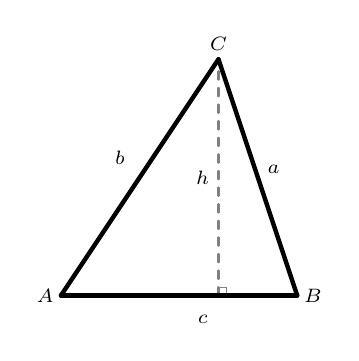
\begin{tikzpicture}[line cap=round]


    \draw [thick, dashed, gray] (2,0) -- (2,3);
    \draw [thin, gray] (2,0.1) -- (2.1,0.1);
    \draw [thin, gray] (2.1,0) -- (2.1,0.1);

	\draw [ultra thick] (0,0) -- (3,0);
	\draw [ultra thick] (3,0) -- (2,3);
	\draw [ultra thick] (0,0) -- (2,3);

 	


	\draw (2.7,1.6) node {\scriptsize{$a$}};
	\draw (0.75,1.75) node {\scriptsize{$b$}};
	\draw (1.8,-0.3) node {\scriptsize{$c$}};
	\draw (1.8,1.5) node {\scriptsize{$h$}};


	\draw (-0.2,0) node {\scriptsize{$A$}};
	\draw (3.2,0) node {\scriptsize{$B$}};
	\draw (2,3.2) node {\scriptsize{$C$}};


    \end{tikzpicture}
  \end{image}

From these two right triangles we can deduce the following. \\

\[    \frac{h}{b} = \sin(A)   \, \text{ and } \,    \frac{h}{a} = \sin(B)       \]



\[    h = b \sin(A)      \, \text{ and } \,    h = a \sin(B)    \]

\[     b \sin(A)  = a \sin(B)    \]


\[    \frac{\sin(A)}{a} = \frac{\sin(B)}{b}      \]




The same argument with an altitude from angle $B$ to side $b$ shows a similar relationship with angle $C$, giving us








\[    \frac{\sin(A)}{a} = \frac{\sin(B)}{b}  = \frac{\sin(C)}{c}    \]
















$\blacktriangleright$  \textbf{\textcolor{blue!55!black}{Obtuse Triangles}}   

An obtuse triangle is one with one angle greater than $90^{\circ}$. 

We can establish the same relationship with an altitude on the outside.








\begin{image}[3in]
    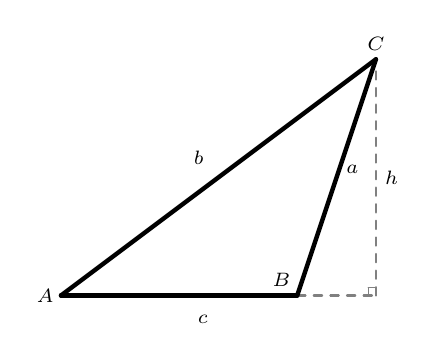
\begin{tikzpicture}[line cap=round]


    \draw [thick, dashed, gray] (4,0) -- (4,3);
    \draw [thick, dashed, gray] (3,0) -- (4,0);
    \draw [thin, gray] (4,0.1) -- (3.9,0.1);
    \draw [thin, gray] (3.9,0) -- (3.9,0.1);

	\draw [ultra thick] (0,0) -- (3,0);
	\draw [ultra thick] (3,0) -- (4,3);
	\draw [ultra thick] (0,0) -- (4,3);

 	


	\draw (3.7,1.6) node {\scriptsize{$a$}};
	\draw (1.75,1.75) node {\scriptsize{$b$}};
	\draw (1.8,-0.3) node {\scriptsize{$c$}};
	\draw (4.2,1.5) node {\scriptsize{$h$}};


	\draw (-0.2,0) node {\scriptsize{$A$}};
	\draw (2.8,0.2) node {\scriptsize{$B$}};
	\draw (4,3.2) node {\scriptsize{$C$}};


    \end{tikzpicture}
  \end{image}











\textbf{Note:}  Straight angles measure $180^{\circ}$.  $\angle B$ is part of a straight angle, which makes the measurement of the angle on the other side $180^{\circ} - B$. 

\textbf{Additional Note:} The $y$-coordinates are the same as you move down the unit circle on either side from $90^{\circ}$.  Therefore, $\sin(180^{\circ} - B) = \sin(B)$ 




\[    \frac{h}{b} = \sin(A)   \, \text{ and } \,    \frac{h}{a} = \sin(180^{\circ} - B)  = \sin(B)      \]



\[    h = b \sin(A)      \, \text{ and } \,    h = a \sin(B)    \]

\[     b \sin(A)  = a \sin(B)    \]


\[    \frac{\sin(A)}{a} = \frac{\sin(B)}{b}      \]




The same argument could be made with angle $C$, giving us








\[    \frac{\sin(A)}{a} = \frac{\sin(B)}{b}  = \frac{\sin(C)}{c}    \]






\begin{theorem}  \textbf{\textcolor{green!50!black}{Law of Sines}} 



For any triangle with angles $A$, $B$, and $C$, and opposite sides $a$, $b$, and $c$, respectively, 


\[    \frac{\sin(A)}{a} = \frac{\sin(B)}{b}  = \frac{\sin(C)}{c}    \]


\end{theorem}





\begin{example}  General Triangles 


Suppose we have a triangle with $A=46^{\circ}$, $B=65^{\circ}$, and $a=14$.

Figure out the other three measurements. (3 decimals)


\textbf{\textcolor{red!75!green}{explanation}} 

$A + B + C = 46^{\circ} + 65^{\circ} + C = \answer{180}^{\circ}$ \\

$C = \answer{69}^{\circ}$


$\frac{\sin(46^{\circ})}{14} = \frac{\sin(65^{\circ})}{b}$

$b = \frac{14 \sin(65^{\circ})}{\sin(46^{\circ})} \approx \answer[tolerance=0.001]{17.63882523}$

$\frac{\sin(46^{\circ})}{14} = \frac{\sin(69^{\circ})}{c}$

$c = \frac{14 \sin(69^{\circ})}{\sin(46^{\circ})} \approx \answer[tolerance=0.001]{18.16961325}$





\end{example}












\begin{example}  No Triangle 


Suppose we have a triangle with $C=55^{\circ}$, $a=4$, and $c=2$.

Figure out the other three measurements.


\textbf{\textcolor{red!75!green}{explanation}} 


$\frac{\sin(55^{\circ})}{2} = \frac{\sin(A)}{4}$

$\sin(A) = \frac{4 \sin(55^{\circ})}{2} \approx 1.638304086$

This is greater than $1$. $\sin(A)$ cannot be greater than $1$.

Therefore, there is no triangle with $C=55^{\circ}$, $a=4$, and $c=2$. 





\end{example}












\begin{example}  Two Triangles 


Suppose we have a triangle with $A=37^{\circ}$, $a=12$, and $b=16$.

Figure out the other three measurements.


\textbf{\textcolor{red!75!green}{explanation}} 


$\frac{\sin(37^{\circ})}{12} = \frac{\sin(B)}{16}$

$\sin(B) = \frac{16 \sin(37^{\circ}}{12}) \approx \answer[tolerance=0.001]{0.8024200309}$

There are two angles whose sine is $0.8024200309$. One in the first quadrant and one in the second quadrant. \\

Therefore, there are two triangles with $A=37^{\circ}$, $a=12$, and $b=16$. 

Using the calculator, the two angles are

\begin{itemize}
\item $B \approx SIN^{-1}(0.8024200309) \approx \answer[tolerance=0.01]{53.36}^{\circ}$
\item $B \approx 180^{\circ} - 53.36^{\circ} = 126.64^{\circ}$
\end{itemize}




\end{example}












































\subsection*{Law of Cosines}
















In the diagram below, we drop an \textbf{altitude} from the top corner (angle $C$). This altitude (length $h$) is perpendicular to the opposite side, forming two right triangles inside the acute triangle. 




\begin{image}[3in]
    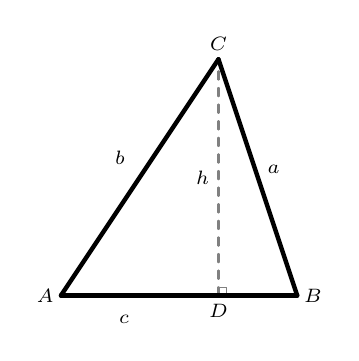
\begin{tikzpicture}[line cap=round]


    \draw [thick, dashed, gray] (2,0) -- (2,3);
    \draw [thin, gray] (2,0.1) -- (2.1,0.1);
    \draw [thin, gray] (2.1,0) -- (2.1,0.1);

	\draw [ultra thick] (0,0) -- (3,0);
	\draw [ultra thick] (3,0) -- (2,3);
	\draw [ultra thick] (0,0) -- (2,3);

 	


	\draw (2.7,1.6) node {\scriptsize{$a$}};
	\draw (0.75,1.75) node {\scriptsize{$b$}};
	\draw (0.8,-0.3) node {\scriptsize{$c$}};
	\draw (1.8,1.5) node {\scriptsize{$h$}};


	\draw (-0.2,0) node {\scriptsize{$A$}};
	\draw (3.2,0) node {\scriptsize{$B$}};
	\draw (2,3.2) node {\scriptsize{$C$}};
	\draw (2,-0.2) node {\scriptsize{$D$}};


    \end{tikzpicture}
  \end{image}




\begin{notation} \textbf{\textcolor{purple!85!blue}{Points, Line Segments, and Lengths}}  

If $A$ and $D$ are two points, then 

\begin{itemize}
\item the actual line segment itself connecting $A$ and $D$ is denoted as $\overline{AD}$. 
\item the length of this line segment is denoted as $m(\overline{AD})$.  $m$ stands for measurement.
\item If $A$ is a point, which is serving as the vertex of an angle, then the angle is denoted by $\measuredangle A$.
\end{itemize}
\end{notation}





From the right triangle on the left in the diagram, we can see that $\cos(\measuredangle A) = \frac{m(\overline{AD})}{b}$ or $m(\overline{AD}) = b \cos(\measuredangle A)$. 


\textbf{Note:} When it is clear, the angle sign is almost always dropped. 


From the right triangle on the left in the diagram, we can see that $\cos(A) = \frac{m(\overline{AD})}{b}$ or $m(\overline{AD}) = b \cos(A)$.


Subtracting this from $m(\overline{AB})$, gives us $m(\overline{DB}) = c - b \cos(A)$.


From the right triangle on the left in the diagram, we can see that $\sin(A) = \frac{h}{b}$ or $h = b \sin(A)$.




From the right triangle on the right in the diagram, the Pythagorean Theorem gives us $a^2 = (b \sin(A))^2 + (c - b \cos(A))^2$.


Multiplying everything out gives


\[    a^2 = b^2 \sin^2(A) +  c^2  - 2 b c \cos(A) + b^2 \cos^2(A)  \]


\[    a^2 = b^2 \sin^2(A) + b^2 \cos^2(A) +  c^2  - 2 b c \cos(A)   \]


\[    a^2 = b^2 (\sin^2(A) + \cos^2(A)) +  c^2  - 2 b c \cos(A)   \]


\[    a^2 = b^2  +  c^2  - 2 b c \cos(A)   \]












\begin{theorem}  \textbf{\textcolor{green!50!black}{Law of Cosines}}  



For any trinagle with angles $A$, $B$, and $C$, and opposite sides $a$, $b$, and $c$, respectively, 


\[    a^2 = b^2  +  c^2  - 2 b c \cos(A)   \]

\[    b^2 = a^2  +  c^2  - 2 a c \cos(B)   \]

\[    c^2 = a^2  +  b^2  - 2 a b \cos(C)   \]


\end{theorem}










\begin{example} Triangle 


Suppose we have a triangle with $a=6$, $b=9$, and $c=11$. Approximate the measurement of angle $A$.

\[    6^2 = 9^2  +  11^2  - 2 \cdot 9 \cdot 11 \cos(A)   \]


\[    \frac{36 - 81 - 121}{- 2 \cdot 9 \cdot 11} =    \cos(A)   \]

\[  \answer[tolerance=0.001]{0.83838383} \approx \cos(A)  \]


\[ A \approx \cos^{-1}(0.83838383)  \approx \answer[tolerance=0.01]{33.030}^{\circ}   \]


\end{example}















































\begin{center}
\textbf{\textcolor{green!50!black}{ooooo-=-=-=-ooOoo-=-=-=-ooooo}} \\

more examples can be found by following this link\\ \link[More Examples of Right Triangles]{https://ximera.osu.edu/csccmathematics/precalculus2/precalculus2/rightTriangles/examples/exampleList}

\end{center}







\end{document}
